\documentclass[a4paper]{article}
\usepackage[
    bookmarks,
    bookmarksopen=true,
    backref,
    plainpages=false,
    pdfpagelabels,
    hypertexnames=false,
    linktocpage,
    colorlinks=true,
    linkcolor=blue,
    anchorcolor=blue,
    citecolor=blue,
    filecolor=blue,
    menucolor=blue,
    urlcolor=cyan,
]{hyperref}
\usepackage{fullpage}
\usepackage{amsmath}
\usepackage{amssymb}
\usepackage{tikz}
\usetikzlibrary{positioning}
\usepackage{booktabs}
\usepackage{verbatim}
\usepackage{hyperref}
\usepackage[parfill]{parskip}
\usepackage[toc,page]{appendix}

\newcommand{\bs}{\boldsymbol}

\newcommand{\Xp}{\bs{\pi}}
\newcommand{\Xps}{\pi^s}

\newcommand{\Xn}{\bs{\nu}^s}
\newcommand{\Xnq}{\nu^s_q}

\newcommand{\Xl}{\Lambda^s}
\newcommand{\Xlp}{\bs{\Lambda}^s_p}
\newcommand{\Xlq}{\bs{\Lambda}^s_{:q}}
\newcommand{\Xlpq}{\Lambda^s_{pq}}
\newcommand{\Xlm}{\overline{\Lambda}^s}
\newcommand{\Xlmp}{\bar{\bs{\Lambda}}^s_p}
\newcommand{\Xlvp}{\Sigma^{p,s}}
\newcommand{\Xlvpi}{\Xlvp{}^{-1}}
\newcommand{\Xlvpll}{\Xlvp_{\Lambda\Lambda}}
\newcommand{\Xlvplu}{\Xlvp_{\Lambda\mu}}
\newcommand{\Xlvpul}{\Xlvp_{\mu\Lambda}}
\newcommand{\Xlvpuu}{\Xlvp_{\mu\mu}}
\newcommand{\Xlvplli}{\Xlvpll{}^{-1}}
\newcommand{\Xlvplui}{\Xlvplu{}^{-1}}
\newcommand{\Xlvpuli}{\Xlvpul{}^{-1}}
\newcommand{\Xlvpuui}{\Xlvpuu{}^{-1}}
\newcommand{\Xlt}{\tilde{\Lambda}^s}
\newcommand{\Xltb}{\tilde{{\bs{\Lambda}}}^s}
\newcommand{\Xltp}{\tilde{\bs{\Lambda}}^s_p}
\newcommand{\Xltpq}{\tilde{\Lambda}^s_{pq}}
\newcommand{\Xltm}{\bar{\tilde{\Lambda}}^s}
\newcommand{\Xltmp}{\bar{\tilde{\bs{\Lambda}}}^s_p}
\newcommand{\Xltmpq}{\bar{\tilde{\Lambda}}^s_{pq}}
\newcommand{\Xltvp}{\tilde{\Gamma}^{p,s}}
\newcommand{\Xltvpi}{\Xltvp{}^{-1}}

\newcommand{\Xu}{\bs{\mu}^s}
\newcommand{\Xup}{\mu^s_p}
\newcommand{\Xum}{\bar{\bs{\mu}}^s}
\newcommand{\Xump}{\bar{\mu}^s_p}

% Data
\newcommand{\Xy}{\bs{y}^n}
\newcommand{\Xs}{s^n}

\newcommand{\Xx}{\bs{x}^n}
\newcommand{\Xxm}{\overline{\bs{x}}^{n,s}}
\newcommand{\Xxv}{\Sigma^s}
\newcommand{\Xxt}{\tilde{\bs{x}}^n}
\newcommand{\Xxtq}{\tilde{x}^n_q}
\newcommand{\Xxtm}{\bar{\tilde{\bs{x}}}^{n,s}}
\newcommand{\Xxtmq}{\bar{\tilde{x}}^{n,s}_q}
\newcommand{\Xxtv}{\tilde{\Sigma}^s}

% Hyperparameters
\newcommand{\Xpsi}{\Psi}
\newcommand{\Xpsii}{\Psi^{-1}}
\newcommand{\Xha}{a^*}
\newcommand{\Xhb}{b^*}
\newcommand{\Xhal}{\alpha^*}
\newcommand{\Xhm}{\bs{m}^*}
\newcommand{\Xhms}{m^*_s}
\newcommand{\Xhu}{\bs{\mu}^*}
\newcommand{\Xhup}{\mu^*_p}
\newcommand{\Xhn}{\bs{\nu}^*}
\newcommand{\Xhnp}{\nu^*_p}

% Operators
\newcommand{\Xcov}{\operatorname{cov}}
\newcommand{\Xvar}{\operatorname{var}}
\newcommand{\Xtr}{\operatorname{tr}}
\newcommand{\Xdiag}{\operatorname{diag}}
\newcommand{\Xvec}{\operatorname{vec}}

% Distributions
\newcommand{\Xdn}{\mathcal{N}}
\newcommand{\Xdm}{\mathcal{M}}
\newcommand{\Xdg}{\operatorname{Ga}}
\newcommand{\Xdd}{\mathcal{D}}



\author{Angermueller Christof}
\date{\today}
\title{Variational Bayesian Mixture of Factor Analysers}

\begin{document}
\maketitle
\tableofcontents

\newpage
\section{Factor analysis}
The factor analysis model describes a $P$ dimensional data vector $\bs{y}$ as a linear function of a $Q$ dimensional vector of latent factors $\bs{x}$ plus some noise $\bs{\eta}$:
\begin{align}
  \bs{y}=\Lambda\bs{x}+\bs{\mu}+\bs{\eta}
\end{align}
The latent factors are assumed to be standard-normal distributed:
\begin{align}
  P(\bs{x})=\mathcal{N}(\bs{x}|0,I_Q)
\end{align}
$\bs{\eta}$ is a normally distributed noise vector with mean zero and diagonal covariance matrix $\Psi$:
\begin{align}
  P(\bs{\eta}|\Psi)=\mathcal{N}(\bs{\eta}|0,\Psi) \qquad
  \Psi=\begin{bmatrix}
    \Psi_{11} & \cdots & 0 \\
    \vdots & \Psi_{ii} & \vdots \\
    0 & \cdots & \Psi_{PP}
  \end{bmatrix}
\end{align}
$\theta=\{\Lambda, \mu, \Psi\}$ are the model parameters. $\Lambda$ is the $P\times Q$ factor loading matrix, whose columns correspond to the eigenvector of the covariance matrix of $\bs{y}$.
Given the latent factors $\bs{x}$, $\bs{y}$ is hence normally distributed itself:
\begin{align}
  P(\bs{y}|\bs{x},\Lambda,\bs{\mu},\Psi)=\mathcal{N}(\bs{y}|\Lambda\bs{x}+\bs{\mu},\Psi)
\end{align}
Integrating out $\bs{x}$ gives:
\begin{align}
  P(\bs{y}|\Lambda,\bs{\mu},\Psi)=\mathcal{N}(\bs{y}|\bs{\mu}, \Lambda\Lambda^T+\Psi)
\end{align}
$\Lambda\Lambda^T+\Psi$ is therefore a low-rank approximation of the full covariance matrix of $\bs{y}$. The factor analysis model is identical to probabilistic Principle Component Analysis (PCA) if $\Psi=\sigma^2 I_P$. Factor analysis is therefore a generalisation for probabilistic PCA, which allows for non-isotropic noise. However, there is no longer a closed-form solution for the maximum likelihood estimator of $\Lambda$.

\subsection{Joint distribution}
\begin{align}
  P(\bs{x}, \bs{y}|\theta)=\mathcal{N}(
  \begin{bmatrix}
  \bs{x} \\ \bs{y} \end{bmatrix} |
  \begin{bmatrix}
    \bs{0} \\
    \bs{\mu}
  \end{bmatrix}),
  \begin{bmatrix}
    I_Q & \Lambda^T \\
    \Lambda & \Lambda\Lambda^T + \Psi
    \label{eq:fa_joint}
  \end{bmatrix}
\end{align}

\subsection{Conditional distributions}
By conditioning on the joint distribution \ref{eq:fa_joint}, one obtains:
\begin{align}
  P(\bs{x}|\bs{y},\theta)=\mathcal{N}(\bs{x}|\Lambda^T(\Lambda\Lambda^T+\Psi)(\bs{y}-\bs{\mu}))
\end{align}
\begin{align}
  P(\bs{y}|\bs{x},\theta)=\mathcal{N}(\bs{y}|\Lambda\bs{x}+\bs{\mu},\Psi)
\end{align}

\subsection{Likelihood}
The log-likelihood of the model parameters $\theta$ is:
\begin{align}
  ll(\theta)=\log\prod_n P(\Xy|\theta)=\sum_n\log \Xdn(\Xy|\Xu,\Xl{\Xl}^T+\Psi)
\end{align}
In contrast to probabilistic PCA, there is no maximum likelihood solution for $\theta$.

\newpage
\section{Mixture of factor analysers}
In the mixture of factor analysers model, $\bs{y}$ belongs to one of $S$ independent factor analysers with different factor loading matrices $\Lambda=\left\{\Xl\right\}_{s=1}^S$ and offset vectors $\bs{\mu}=\left\{\Xu\right\}_{s=1}^S$:
\begin{align}
  \bs{y}=\Xl\bs{x}+\Xu+\bs{\eta}
\end{align}
The indicator $s$ is unknown and therefore integrated out:
\begin{align}
  P(\bs{y}|\theta)=\sum_s P(s|\Xp)P(\bs{y}|s,\theta)=\sum_s P(s|\Xp)\Xdn(\bs{y}|\Xu\Xl{\Xl}^T+\Psi)
\end{align}
The prior $P(\bs{s}|\Xp)$ is a single draw from a multinomial distribution with mixture-coefficients $\Xp$:
\begin{align}
  P(\bs{s}|\Xp)=\Xdm(\bs{s}|1,\Xp)
\end{align}
The model parameters $\theta=\left\{\Xp,\Lambda,\bs{\mu},\Psi\right\}$ can estimated by maximum likelihood or Bayesian inference. Maximum likelihood estimation via Expectation Maximisation (EM) is fast, but subject to overfitting since it does not take into account model complexity. Bayesian inference prevents overfitting by imposing a prior on the model parameters, but is often intractable. To make inference tractable, approximate Bayesian inference methods can be used. The following sections will explain one of these methods, Variational Inferece, which allows for tractable inference for a Bayesian mixture of factor analysers.

\newpage
\section{Variational Bayesian mixture of factor analysers}
\subsection{Prior distribution}
Bayesian inference requires a prior distribution $P(\theta)$ over the model parameters $\theta=\left\{\Xp,\Lambda,\bs{\mu}\right\}$, which can be chosen as follows.

The prior over the mixture proportions $\bs{\pi}$ is a symmetric Dirichlet distribution with counts $\Xhal\Xhm$:
\begin{align}
  P(\Xp|\Xhal\Xhm)=\Xdd(\Xp|\Xhal\Xhm),
\end{align}
The prior strengths $\Xhal$ corresponds to the total number of prior counts, and $\Xhm$ to the prior distribution, which is supposed to be uniform: $\Xhm=[1/S,\dots,1/S]$.
The expectation and variance is therefore:
\begin{align}
  <\pi_s>=m_s \qquad \Xvar[\pi_s]=\frac{m_s(1-m_s)}{\Xhal(\Xhal+1)}
\end{align}

Each factor loading matrix $\Xl$ factorizes by columns $q$, which are normally distributed with mean zero and diagonal covariance matrix ${\Xnq}^{-1}I_P$. This is equivalent to saying $\Xl$ factorizes by rows $p$, which are normally distributed with mean zero and diagonal covariance matrix $\Xdiag[\Xn]^{-1}$.
\begin{align}
  P(\Lambda|\bs{\nu})&=\prod_{s,q}\Xdn(\Xlq|0,{\Xnq}^{-1}I_P) \\
                &=\prod_{s,p}\Xdn(\Xlp|0,\Xdiag[\Xn]^{-1})
\end{align}

The factor loading rates $\Xn$ are independently Gamma distributes with hyperparameter $\Xha$ and $\Xhb$:
\begin{align}
  P(\bs{\nu}|\Xha,\Xhb)=\prod_{s,q}\Xdg(\Xnq|\Xha,\Xhb)
\end{align}

The mean vector $\Xu$ is normally distributed with mean $\Xhu$ and diagonal covariance $\Xdiag[\Xhn]^{-1}$:
\begin{align}
  P(\bs{\mu}|\Xhu,\Xhn)=\prod_s\Xdn(\Xu|\Xhu,\Xdiag[\Xhn]^{-1})
\end{align}

In summary, the model parameters $\theta$ are
\begin{align}
  \theta=\left\{\Xp,\bs{\nu},\Lambda,\bs{\mu}\right\},
\end{align}
and the hyperparameters $\Theta$ are
\begin{align}
  \Theta=\left\{\Xpsi,\Xhal\Xhm,\Xha,\Xhb,\Xhu,\Xhn\right\}.
\end{align}

\subsection{Joint distribution}
The data $D$ includes the observed variables $\Xy$, as well as the latent variables $\Xx$ and $\Xs$ for $n=1,\dots,N$ independent samples:
\begin{align}
  D=\left\{\Xy,\Xx,\Xs\right\}_{n=1}^N
\end{align}
The joint distribution of model parameters $\theta$ and data $D$ factorises as follows:
\begin{align}
  P(\theta,D|\Theta)&=P(\theta|\Theta)P(D|\theta,\Theta) \\
  &=P(\Xp|\Xhal\Xhm)P(\bs{\nu}|\Xha,\Xhb)P(\Lambda|\bs{\nu})P(\bs{\mu}|\Xhu,\Xhn) \\
  &\quad \prod_n P(\Xs|\Xp)P(\Xx)P(\Xy|\Xx,\Xl,\Xu,\Xpsi)
\end{align}
The log joint distribution is:
\begin{align}
  \log P(\theta,D|\Theta)&= \log P(\theta|\Theta) + \log P(D|\theta,\Theta) \\
  &=\log P(\Xp|\Xhal\Xhm) + \log P(\bs{\nu}|\Xha,\Xhb) + \log P(\Lambda|\bs{\nu}) + \log P(\bs{\mu}|\Xhu,\Xhn) \\
  &\quad \sum_n \log P(\Xs|\Xp) + \log P(\Xx) + \log P(\Xy|\Xx,\Xl,\Xu,\Xpsi)
  \label{eq:log_joint}
\end{align}

\begin{figure}[h]
  \begin{center}
    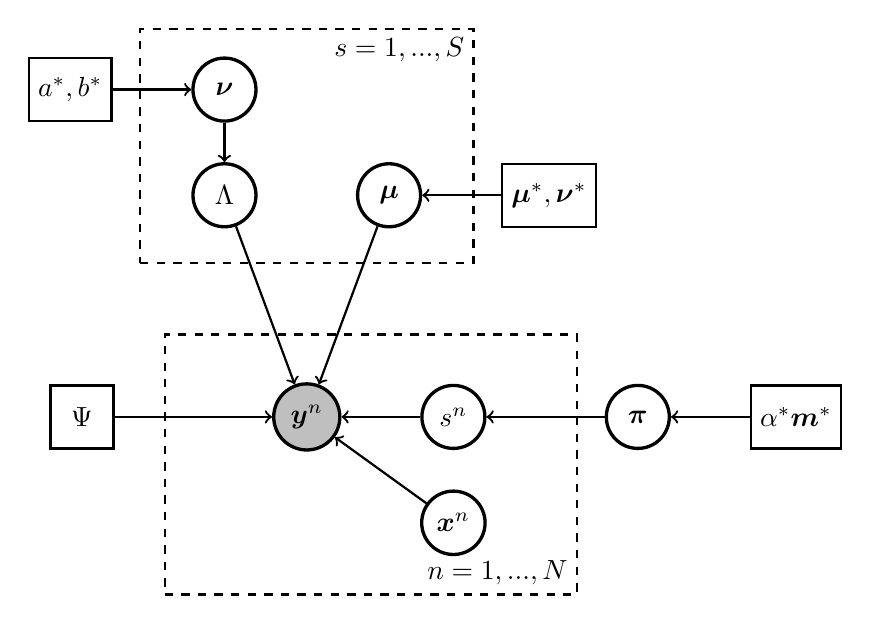
\begin{tikzpicture}
      \tikzstyle{sVar}=[circle, draw=black, very thick, minimum size=.8cm];
      \tikzstyle{sPlate}=[rectangle, dashed, draw=black, thick, align=flush right];
      \tikzstyle{sHyper}=[rectangle, draw=black, thick, minimum size=.8cm];
      \tikzstyle{sDep}=[->, thick];
      \node[sPlate, text width=5cm, text height=3cm] (Pn) {$n=1,...,N$};
      \node[sVar, below left=.75cm and .5cm of Pn.north, fill=gray!50] (Y) {$\Xy$};
      \node[sVar, right=1cm of Y] (Z) {$\Xs$};
      \node[sVar, below=.5cm of Z] (X) {$\Xx$};
      \node[sVar, right=1.5cm of Z] (Pi) {$\Xp$};
      \node[sHyper, left=2cm of Y] (Psi) {$\Xpsi$};
      \node[sHyper, right=1cm of Pi] (Alpha) {$\alpha^*\bs{m}^*$};
      \node[sPlate, align=flush right, text width=4cm, text depth=2.5cm, above=1.5cm of Y] (Ps) {$s=1,...,S$};
      \node[above =.75cm of Ps.south] (Sh) {};
      \node[sVar, left=.5cm of Sh] (L) {$\Lambda$};
      \node[sVar, above=.5cm of L] (Nu) {$\bs{\nu}$};
      \node[sVar, right=.5cm of Sh] (Mu) {$\bs{\mu}$};
      \node[sHyper, right=1cm of Mu] (MuH) {$\bs{\mu}^*,\bs{\nu}^*$};
      \node[sHyper, left=1cm of Nu] (NuH) {$a^*,b^*$};
      \draw[sDep] (Z) -- (Y);
      \draw[sDep] (X) -- (Y);
      \draw[sDep] (Psi) -- (Y);
      \draw[sDep] (Pi) -- (Z);
      \draw[sDep] (Alpha) -- (Pi);
      \draw[sDep] (L) -- (Y);
      \draw[sDep] (Mu) -- (Y);
      \draw[sDep] (Nu) -- (L);
      \draw[sDep] (NuH) -- (Nu);
      \draw[sDep] (MuH) -- (Mu);
    \end{tikzpicture}
    \caption{Graphical model}
  \end{center}
\end{figure}

\newpage
\section{Variational approximation}
The goal is to approximate the following posterior distribution:
\begin{align}
  P(\bs{\pi},\bs{\nu},\Lambda,\bs{\mu},\bs{x},\bs{s}|\bs{y}) \approx Q(\bs{\pi},\bs{\nu},\Lambda,\bs{\mu},\bs{x},\bs{s})
\end{align}
To render tractable inference and closed form solutions for the approximating factors $Q(\cdot)$, the following factorisation is chosen:
\begin{align}
  Q(\bs{\pi},\bs{\nu},\Lambda,\bs{\mu},\bs{x},\bs{s})=Q(\bs{\pi},\bs{\nu})Q(\Lambda,\bs{\mu})Q(\bs{x},\bs{s})
\end{align}
The choice of this factorisation implies two approximations:
\begin{enumerate}
  \item Parameters $\theta$ and latent variables $\left\{\bs{x},\bs{s}\right\}$ are independent.
  \item $\left\{\Lambda,\bs{\mu}\right\}$ are independent of the remaining parameters.
\end{enumerate}
The optimal $Q(\cdot)$ can be found be computing the expectation of the log joint distribution (eq.~\ref{eq:log_joint}):
\begin{align}
  \log Q_i \propto <\log P(\theta,D|\Theta)>_{Q_{-i}}
\end{align}
This leads to the following factorization:
\begin{align}
  Q(\bs{\pi},\bs{\nu})Q(\Lambda,\bs{\mu})Q(\bs{x},\bs{s})=Q(\bs{\pi})\prod_s\prod_q Q(\nu_q^s)\prod_s\prod_p Q(\tilde{\Lambda}^s_p) \prod_n Q(\Xx|\Xs)Q(\Xs)
\end{align}
Here, $\Xlt$ is the concatenation of $\Xl$ and $\bs{\mu}^s$:
\begin{align}
  \Xlt:=[\Xl \: \Xu].
\end{align}
The factors are distributed as follows:
\begin{align}
  Q(\Xp)=\mathcal{D}(\Xp|\alpha\bs{m})
\end{align}
\begin{align}
 Q(\nu^s_q)=\mathcal{G}(\nu^s_q|a, b_q^s)
\end{align}
\begin{align}
  Q(\Xltp)=\mathcal{N}(\Xltp|\Xltmp,\Xltvp)
\end{align}
\begin{align}
  Q(\Xx|\Xs)=\mathcal{N}(\Xx|\Xxm,\Xxv)
\end{align}
\begin{align}
  Q(\Xs)\text{ is }N\times S
\end{align}

\subsection{$Q(\Xp)$}
\begin{align}
  Q(\Xp)=\mathcal{D}(\Xp|\alpha\bs{m})
\end{align}
\begin{align}
  \alpha m_s=\Xhal\Xhms+\sum_n Q(\Xs)
\end{align}

\subsection{$Q(\Xnq)$}
\begin{align}
 Q(\Xnq)=\mathcal{G}(\Xnq|a, b_q^s)
\end{align}
\begin{align}
a&=a^*+\frac{P}{2} \\
b_q^s&=b^*+\frac{1}{2}\sum_p<\Xlpq{}^2> \\
&=b^*+\frac{1}{2}\sum_p\left(\Xltmpq{}^2 + \Xltvp_{qq}\right)
\end{align}
Here, we solved $<\Xltpq{}^2>$ by eq.~\ref{eq:x2}.

\subsection{$Q(\Xltp)$}
\begin{align}
  Q(\Xltp)=\mathcal{N}(\Xltp|\Xltmp,\Xltvp)
\end{align}
The extended loading matrix $\Xlt$ is $P\times (Q+1)$ and factorizes over rows:
\begin{align}
  \Xlt=\left[
    \begin{array}{ccc|c}
      \Xl_{11} & \cdots & \Xl_{1Q} & \mu^s_1 \\
      \vdots & \vdots & \vdots & \vdots \\
      \Xl_{p1} & \cdots & \Xl_{pQ} & \mu^s_p \\
      \vdots & \vdots & \vdots & \vdots \\
      \Xl_{P1} & \cdots & \Xl_{PQ} & \mu^s_P
    \end{array}
  \right]
\end{align}
The row mean is $(Q+1)\times 1$:
\begin{align}
  \Xltmp=\begin{bmatrix}
    \Xlmp \\
    \Xump
  \end{bmatrix}
\end{align}
\begin{align}
  \Xlmp
  &=\Xltvp_{\Lambda\Lambda}\left(\Xpsii_{pp}\sum_n Q(\Xs)y^n_p<\Xx>\right) \\
  &=\Xltvp_{\Lambda\Lambda}\left(\Xpsii_{pp}\sum_n Q(\Xs)y^n_p\Xxm\right)
\end{align}
\begin{align}
  \Xump
  &=\Xltvp_{\mu\mu}\left(\Xpsii_{pp}\sum_n Q(\Xs)y^n_p+\nu^*_p\mu^*_p\right)
\end{align}
The row covariance matrix is $P\times(Q+1)$ and decomposes into $4$ blocks:
\begin{align}
  \Xltvpi=\begin{bmatrix}
    \Xlvplli & \Xlvplui \\
    \Xlvpuli & \Xlvpuui
  \end{bmatrix}
\end{align}
$\Xlvpll$ is $Q\times Q$:
\begin{align}
  \Xlvplli
  &=\Xdiag[<\Xn>]+\Xpsii_{pp}\sum_n Q(\Xs)<\Xx{\Xx}^T> \\
  &=\Xdiag[\frac{a}{b^s_1},...,\frac{a}{b^s_Q}]+\Xpsii_{pp}\sum_n Q(\Xs)\left(\Xxm{\Xxm}^T+\Xxv\right) \label{eq:ulvppli}
\end{align}
Eq.~\ref{eq:ulvppli} follows from eq.~\ref{eq:xx}. \\
$\Xlvplui$ is $Q\times 1$:
\begin{align}
  \Xlvplui
  &=\Xpsii_{pp}\sum_n Q(\Xs)<\Xx> \\
  &=\Xpsii_{pp}\sum_n Q(\Xs)\Xxm
\end{align}
$\Xlvpuu$ is $1\times 1$:
\begin{align}
  \Xlvpuui&=
  \nu^*_p+\Xpsii_{pp}\sum_n Q(\Xs)
\end{align}

\subsection{$Q(\Xx|\Xs)$}
\begin{align}
  Q(\Xx|\Xs)=\mathcal{N}(\Xx|\Xxm,\Xxv)
\end{align}
\begin{align}
  \Xxm
  &=\Xxv<{\Xl}^T\Xpsii(\Xy-\Xu)> \\
  &=\Xxv\left[{\Xlm}^T\Xpsii\left(\Xy-\Xum\right)-\bs{v}\right] \label{eq:uxxm}
\end{align}
Eq.~\ref{eq:uxxm} follows from eq.~\ref{eq:XAy} and $\bs{v}$ is defined as
\begin{align}
  v_q
  &=\Xtr[\Xpsii\Xcov[\Xl_{:q},\Xu]] \\
  &=\sum_p \Xpsii_{pp} {\Xlvplu}_q. \label{eq:uxxmv}
\end{align}
Eq.~\ref{eq:uxxmv} follows from $\Xcov[\Xl_{pq},\mu^s_{p^\prime}]=0$ if $p\neq p^\prime$ and $\Xcov[\Xl_{pq},\mu^s_{p}]={\Xlvplu}_q$.
\begin{align}
  {\Xxv}^{-1}=<{\Xl}^T \Xpsii \Xl>+I
\end{align}
$<{\Xl}^T \Xpsii \Xl>$ is solved by eq. $\ref{eq:XAY}$ and $\Xcov[\Xl_{pi},\Xl_{p^\prime j}]=0$ for $p\ne p^\prime$:
\begin{align}
  <{\Xl}^T \Xpsii \Xl>_{ij}&=<{\Xl_{:i}}^T \Xpsii \Xl_{:j}> \\
  &=<\Xl_{:i}>^T\Xpsii <\Xl_{:j}>+\sum_p\sum_{p^\prime} \Xpsii_{pp^\prime}\Xcov[\Xl_{pi},\Xl_{p^\prime j}] \\
  &=<\Xl_{:i}>^T\Xpsii <\Xl_{:j}>+\sum_p \Xpsii_{pp}\Xcov[\Xl_{pi},\Xl_{pj}] \\
  &={\Xlm_{:i}}^T\Xpsii \Xlm_{:j}+\sum_p \Xpsii_{pp}{\Xlvpll}_{ij}
\end{align}

\subsection{$Q(\Xs)$}
\newcommand{\Xsvv}{\bs{\sigma}^{s,n}}
\newcommand{\Xsvm}{C_{\Xlt}}
\begin{align}
  \ln Q(\Xs)
  &=\psi(\alpha m_s)+\frac{1}{2}\ln |\Xxv|+<\ln P(\Xy|\Xx,\Xs,\Xl,\Psi)> \label{eq:usqe} \\
  &=\psi(\alpha m_s)+\frac{1}{2}\ln |\Xxv| \nonumber \\
  &\quad-\frac{1}{2}(\Xy-\Xltm\Xxtm)^T\Xpsii(\Xy-\Xltm\Xxtm) \nonumber \\
  &\quad-\frac{1}{2}\Xdiag[\Xpsii]^T \Xsvv
\end{align}
Here, the following definitions were used:
\begin{align}
  \Xxt &= [\Xx \quad 1]^T \\
  \Xsvv &= (\Xltm{}^2+\Xsvm)\Xdiag[\Xxtv]+ \Xsvm \Xxtm{}^2 \\
  \Xsvm &= \begin{bmatrix}
    \Xdiag[\tilde{\Gamma}^{1,s}]^T \\
    \cdots \\
    \Xdiag[\tilde{\Gamma}^{P,s}]^T \\
  \end{bmatrix}
\end{align}
The expectation in eq.~\ref{eq:usqe} is:
\begin{align}
  <\ln P(\Xy|\Xx,\Xs,\Xl,\Psi)> \\
  &=-\frac{1}{2}<(\Xy-\Xlt\Xxt)^T\Xpsii(\Xy-\Xlt\Xxt)> + \text{const} \\
  &=-\frac{1}{2}(\Xy-\Xltm\Xxtm)^T\Xpsii(\Xy-\Xltm\Xxtm)
  -\frac{1}{2}\Xtr[\Xpsii \Xvar[\Xlt\Xxt]] + \text{const}
\end{align}
\begin{align}
  \Xvar[\Xlt\Xxt]=
  \begin{bmatrix}
    \Xvar[\Xltb_1{}^T\Xxt] & \cdots & 0 \\
    \cdots & \Xvar[\Xltb_p{}^T\Xxt] & \cdots \\
    0   & \cdots & \Xvar[\Xltb_P{}^T\Xxt]
  \end{bmatrix}
\end{align}
\begin{align}
  \Xvar[\Xltp{}^T\Xxt]
  &=\sum_q\Xvar[\Xltpq\Xxtq] \\
  &=\sum_q<\Xltpq{}^2><\Xxtq{}^2>-<\Xltpq>^2<\Xxtq>^2 \label{eq:usv1} \\
  &=\sum_q(<\Xltpq>^2+\Xvar[\Xltpq])(<\Xxtq>^2+\Xvar[\Xxtq])-<\Xltpq>^2<\Xxtq>^2 \label{eq:usv2} \\
  &=\sum_q<\Xltpq>^2\Xvar[\Xxtq]+<\Xxtq>^2\Xvar[\Xltpq]+\Xvar[\Xltpq]\Xvar[\Xxtq] \\
  &=\sum_q\Xltmpq{}^2\Xxtv_{qq}+\Xxtmq{}^2\Xltvp_{qq}+\Xltvp_{qq}\Xxtv_{qq} \\
  &=\sum_q(\Xltmpq{}^2+\Xltvp_{qq})\Xxtv_{qq}+\Xxtmq{}^2\Xltvp_{qq}
\end{align}
\begin{align}
  \Xvar[\Xlt\Xxt] &= \Xdiag[\Xsvv]
\end{align}
\begin{align}
  \Xtr[\Xpsii \Xvar[\Xlt \Xx]] = \Xdiag[\Xpsii]^T \Xsvv \label{eq:usv3}
\end{align}


\begin{appendices}

\section{Expectations}
\newcommand{\Xvx}{\bs{x}}
\newcommand{\Xvy}{\bs{y}}

\begin{align}
  \label{eq:x2}
  <\bs{x}^2>=<\bs{x}>^2+\Xvar[\bs{x}]
\end{align}
\begin{align}
  \label{eq:xAx}
  <\bs{x}^T A \bs{x}>=<\bs{x}>^T A <\bs{x}> + \Xtr[A \Xvar[\bs{x}]]
\end{align}
\begin{align}
  \label{eq:xAy}
  <\bs{x}^T A \bs{y}>
  &=<\bs{x}>^T A <\bs{y}> + \Xtr[A \Xcov[\bs{y},\bs{x}]] \\
  &=<\bs{x}>^T A <\bs{y}> + \Xvec[A]^T\Xvec[\Xcov[\bs{x},\bs{y}]]
\end{align}
\begin{align}
  \label{eq:XAY}
  <X A Y>&=<X>A<Y>+V \\
  V_{ij}&=\Xtr[A\Xcov[Y_{:j},X_i]]=\Xvec[A]^T\Xvec[\Xcov[X_i,Y_{:j}]] \nonumber
\end{align}
\begin{align}
  \label{eq:XAy}
  <X A \bs{y}>&=<X>A<\bs{y}>+\bs{v} \\
  \bs{v}_{i}&=\Xtr[A\Xcov[\bs{y},A_i]]=\Xvec[A]^T\Xvec[\Xcov[X_i,\bs{y}]] \nonumber
\end{align}
\begin{align}
  \label{eq:xx}
  <\bs{x}\bs{x}^T>=<\bs{x}><\bs{x}>^T+ \Xcov[\bs{x}]
\end{align}
If $M$ and $\Xvx$ are independent:
\begin{align}
  \label{eq:Mx}
  <M \Xvx>=<M><\Xvx>
\end{align}
If $\Xvx$ and $\Xvy$ are independent:
\begin{align}
  \Xvar[\Xvx^T\Xvy]
  &=\sum_i \Xvar[\Xvx_i \Xvy_i] \nonumber\\
  &=\sum_i <\Xvx_i^2><\Xvy_i^2> - <\Xvx_i>^2<\Xvy_i>^2 \label{eq:vxy}
\end{align}

\end{appendices}


\end{document}
